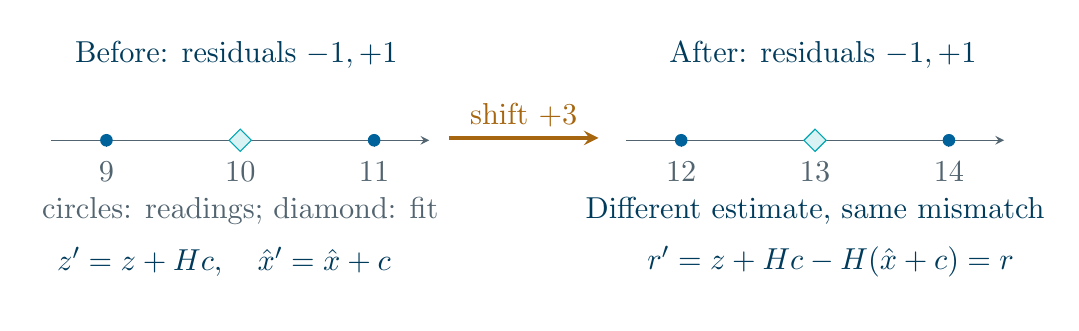
\begin{tikzpicture}[x=1cm,y=1cm,font=\fontsize{11}{13}\selectfont,>=stealth]
\definecolor{IEEEBlue}{HTML}{00629B}
\definecolor{Cyan}{HTML}{00A6B2}
\definecolor{Navy}{HTML}{003B5C}
\definecolor{Slate}{HTML}{526470}
\definecolor{Amber}{HTML}{A66610}
\path[use as bounding box] (0,0) rectangle (13,3.5);
\node[text=Navy] at (2.65,3.16) {Before: residuals $-1,+1$};
\node[text=Navy] at (10.1,3.16) {After: residuals $-1,+1$};
\draw[->,Slate] (.3,2.07)--(5.1,2.07);
\draw[->,Slate] (7.6,2.07)--(12.4,2.07);
\foreach \x/\v in {1/9,2.7/10,4.4/11,8.3/12,10/13,11.7/14} {\draw[Slate] (\x,1.99)--(\x,2.15);\node[below,text=Slate] at (\x,1.92) {\v};}
\foreach \x in {1,4.4,8.3,11.7} {\fill[IEEEBlue] (\x,2.07) circle (.08);}
\foreach \x in {2.7,10} {\node[draw=Cyan,fill=Cyan!15,minimum size=.2cm,rotate=45,inner sep=0pt] at (\x,2.07) {};}
\draw[->,Amber,line width=1.3pt] (5.35,2.1)--node[above,text=Amber] {shift $+3$} (7.25,2.1);
\node[text=Slate] at (2.7,1.17) {circles: readings; diamond: fit};
\node[text=Navy] at (10,1.17) {Different estimate, same mismatch};
\node[anchor=west,text=Navy] at (.25,.53) {$z'=z+Hc,\quad\hat x'=\hat x+c$};
\node[anchor=east,text=Navy] at (12.65,.53) {$r'=z+Hc-H(\hat x+c)=r$};
\end{tikzpicture}%
